\message{ !name(Ch1b.tex)}
\message{ !name(Ch1b.tex) !offset(-2) }
\chapter{
Models for Spatial Capture-Recapture Data
}
\markboth{Modeling}{}
\label{chapt.modeling}


\vspace{.3in}

In the previous chapter we described basic concepts of
capture-recapture methods, and explained the limitations of
non-spatial models. In this
chapter we lay out our approach to modeling spatial capture-recapture
data, but first we introduce notation and basic statistical
concepts. We focus on concepts that are simple but critical to an
understanding of the material presented in the remainder of this
book. Some of these are concepts
are so elemetary that we fear some might take offense, but our
experience is that many introductory statistics
courses offered to ecologists do not adequately impart these
fundamentals. Instead, there seems to be much attention paid to
minor details such as computing the number of degrees of freedom in
various $F$-tests. In addition to being basic, all of the material in the
beginning of this chapter is explained in numerous other texts, but we present it here
using examples relevant to SCR. Futhermore, we emphasize the use of
\R~as a hands-on teaching tool. We encourage readers that seek a deeper and more
technical treatment of these ideas to consult
\citet{williams_etal:2002}, \citet{royle_dorazio:2008} and
\citet{link_barker:2010}. \citet{mackenzie_etal:2005} is another
slightly less technical reference with ecological examples.

\section{Random Variables and Probability Distributions}

A random variable is what its name implies---a variable whose
value is the outcome of some stochasitic process. One source
of stochasticity inherent to virtually all ecological data
results from sampling a population. A sample of data can be
regarded as a random variable because the data will typically differ from
other samples unless the sample size is close to the population size or the
variance of the population is negligible.
Because the estimates sample data are random variables, sample
statistics are also random variables.
Sampling variation is
often regarded as a nuicance. We might wish it were otherwise.

To adequately characterize how our data arise, we need a hypothesis
written in mathmatical terms---we need a statistical
model.


To characterize both the uncertainty in our data and in our estimates
of population parameters, we need a model.

To describe our understanding of how the data arose, we need a
model. A model simply embodies our hypotheses about the system in some
quantitative way. For example, a simple model for our shad length data
is to assume that they arose from a normal distribution whose mean and
variance correspond to the mean and variance of the population. If
mean shad length is $\mu$=60cm with variance $\sigma^2$=10cm, the

As an extremely simplistic
example, imagine that we
caught 50 American shad (\emph{Alosa sapidissima}) from the secret shad
hole on Deerfield River in Massachusetts and we
measure the length of each individual. When the shadberry (\emph{Amelanchier
  arborea} is in bloom, the shad are so bountiful and
variable that it is very unlikely that a second sample
of fish will have the same lengths as the first.
For example, suppose we caught
our 50 shad because we wanted to estimate the average length of shad in
the pool. The average fish length of the entire population is a
parameter, and the average fish length in our sample is a statistic
that can regarded as an estimate of that parameter. If we repeatedly
sample the population, the sample statistic will vary but the
population parameter will not, assuming the fish aren't growing during
the sampling period.




Most
random variables can be regarded as continuous or discrete. Shad length is an
example of a continuous random variable.

For example, if we wish to know
the average length of fish in the sea, we might catch 100 of them and
record their lengths. If we throw them back and
collect a new sample the next day, our second sample will almost
certainly differ from the first

If $y$ is the length of a fish captured in a river, we
would expect this value to differ with each new sample from the
population inhabiting the river. Fish length is an example of a
continuous random variable.


\section{Models for Random Variables}





\section{Modeling Phiolosophy}

In this book we present a diverse array of modeling approaches for making
inference about density and population dynamics using spatial
capture-recapture data. A number of conceptual and
methodological themes unify the main topical coverage of this book, and
those are:

\begin{itemize}
\item[(1)] Hierarchical modeling. We develop hierarchical models
  consisting of explicit models for both the observation process and
  the underlying ``ecological process'' which describes the
  organization of individuals in space.

\item[(2)] Formal inference using both classical (frequentist,
  likelihood-based) and Bayesian methods. We often emphasize
  Bayesian analysis because this allows us to focus the technical
  formulation of models, and spatial capture-recapture is mainly
  concerned with modeling random effects and estimating functions of
  random effects. However, we also explore likelihood methods using existing
  software such as the R package SECR \citep{efford:2011}, as well as
  development of custom solutions along the way.

\item[(3)] In developing Bayesian analyses of SCR models, we emphasize
  the use of the BUGS language for describing models. The BUGS
  language emphasizes the syntactic description of the essential
  assumptions of models in a special kind of pseudo-code language,
  which is used in software (WinBUGS, JAGS, OpenBUGS) to devise Markov
  chain Monte Carlo (MCMC) algorithms for Bayesian analysis of
  models. The BUGS language focuses your thinking on model development
  and lets you develop an understanding of models at the level of
  their basic assumptions and structure.  Despite our focus on
  describing models using the BUGS language, we also show readers how
  to devise their own MCMC algorithms for Bayesian analysis of SCR
  models, which can be convenient (even necessary) in some practical
  situations.

\item[(4)] Data augmentation -- dealing with the fact that population
  size, $N$, is unknown is a challenging technical problem in
  capture-recapture models. We confront this problem in almost every
  chapter of this book. To deal with it we use a technical device
  called {\it data augmentation} which is extremely useful for
  analysis of capture-recapture models that are specified
  ``conditional on $N$'' \citep{royle_etal:2007}.
\end{itemize}

Altogether, these different conceptual and methodological elements
provide for a formulation of SCR models that essentially renders them
as variations of generalized linear mixed models (GLMMs). This in a
sense makes them consistent with many important methodologies used in
ecology (e.g., see \citet{zuur_etal:2009, kery_etal:2010}), and
because of the connection with standard modeling concepts, we believe
that the material presented in this book can be understood and used by
most ecologists with some modeling experience.

This book is not a book about Bayesian analysis, not a book about
hierarchical models, not a book about capture-recapture, and not about
programming in R. In a sense though, our book integrates elements of
all of these things into what we hope is a coherent package for
analyzing data from this enormous class of data collection methods
that produce spatially-explicit capture-recapture data.   As such, we
expect that people have a basic understanding of statistical models
and classical inference (What is frequentist inference? what is a
likelihood? Generalized linear model? Generalized linear mixed
model?),
{\bf R} programming,
 Bayesian analysis (what is s a prior distribution and a
posterior distribution?),
and maybe even a little bit
of Bayesian
computation (MCMC and perhaps the BUGS language).
The ideal candidate for reading this book has basic knowledge of these
topics. However, we do provide introductory chapters on the necessary
components which we hope can serve as a brief and cursory tutorial for
those who might have only limited technical knowledge, e.g., many
carnivore biologists who implement field sampling programs but do not
have extensive experience analyzing data.


\section{Key Concepts in Statistical Modeling}

We should cover a few basic topics like:

random variables

distributions

likelihood

estimates and estimators

confidence intervals




\section{Hierarchical Models and Inference}

The term hierarchical modeling (or hierarchical model) has become
something of a buzzword over the last decade with hundreds of papers
published in ecological journals using that term.  So then, what
exactly is a hierarchical model, anyhow? Obviously, this term stems
from the root ``hierarchy'' which means:

\vspace{.1in}

{\flushleft
Definition: {\it hierarchy} (noun) -- a series of ordered groupings of people or things within a system;
}

\vspace{.1in}

In the case of a hierarchical model (hierarchical being the adjective
form of hierarchy), the ``things'' are probability distributions, and
they are ordered according to their conditional probability structure.
Thus, a hierarchical model is {\it an ordered series of models,
  ordered by their conditional probability structure}.

If we declare that the random variable $y = $ \# of times an
individual is encountered in a trap out of $K=10$ days has a
$\mbox{Bin}(10, p)$ distribution then this is but a single model and,
thus, not a hierarchical model. If, however, we declare that
\[
y \sim \mbox{Bin}(10,p)
\]
{\it and}
\[
p \sim \mbox{beta}(1,1)
\]
which is the same as the previous model but with a ``flat'' prior
distribution on $p$, then this is kind of a cheap pedestrian
hierarchical model according to our definition although it is barely
more interesting than the previous non-hierarchical model.
%% I think here in the intro you could remove this 'pedestrian hierarchical model'
%% For the readers who are not familiar (yet) with distributions and what a prior is, I think it would be mroe helpful
%% to only use the following example and explain briefly what the
%% p_{i}\sim \mbox{beta}(\mu, \tau) stands for
On the
other hand, suppose we have some meaningful group structure in this
problem such that the data arise by observing repeated Bernoulli
trials on {\it individuals}, e.g., they are eggs hatching from a
common nest (or parentage). So let $y_{i}$ be the outcomes for
individuals $i=1,2,...,N$ with
\[
y_{i} \sim \mbox{Bin}(K, p_{i})
\]
 and
\[
p_{i}\sim \mbox{beta}(\mu, \tau).
\]
Because of the meaningful group structure, this is a more interesting
hierarchical model. In fact, in the context of capture-recapture this
is a specific version of ``Model Mh'' (see Chapt. 3 and
\citet{dorazio_royle:2003}).  We should consider this a type of a
hierarchical model although we will make a further conceptual
distinction shortly that further dichotimizes the space of
hierarchical models.

A canonical hierarchical model in ecology is this
elemental model of species occurrence or distribution
\citep{mackenzie_etal:2002, tyre_etal:2003, kery:2011}:
\[
y_{i}|z_{i} \sim \mbox{Bin}(K,z_{i} \,  p)
\]
\[
z_{i} \sim \mbox{Bern}(\psi)
\]
where  $y_{i} = $ observation of presence/absence at a site $i$ and
$z_{i} = $ occurrence status ($z_{i}=1$ if a species occurs at  site
$i$ and $z_{i}=0$ if not).  This model has an important conceptual
distinction between the hierarchical model shown just previously
(Model Mh) and also other types of classical multi-level models such
as repeated measures on subjects, in that $z_{i}$ is an actual state
of nature. In that sense, $z$ is a random variable that is the outcome of a
``real'' process.   \citet{royle_dorazio:2008} used the term {\it
  explicit} hierarchical model to describe this type of model to
distinguish from hierarchical models ({\it implicit} hierarchical
models) where the latent variables don't
correspond to an actual state of nature -- but rather just soak up
variation that is unmodeled by explicit elements of the model.
At best, latent variables in such models
are a a surrogate for something of ecological relevance
(``time effects'', ``space effects'' etc.).


With these examples,
we expand on our definition of a hierarchical model as we will use it
in this book: \newline
{\flushleft {\bf Definition}: {\it Hierarchical Model}: A model with
  explicit component models that describe variation in the data due to
  (spatial/temporal) variation in {\it ecological process}, and due to
  {\it imperfect observation} of the process.
}



%\subsection{Anatomy of a hierarchical model}
%Interesting hierarchical models in ecology typically
%contain the following components:
%\begin{itemize}
%\item[{\bf 1.}] {\it Observations}, $y(s,t)$ -- ``data''
%\item[{\bf 2.}] {\it Observation model} $[y|z,\theta_1]$
%\item[{\bf 3.}] {\it State variable}, $z(s,t)$: outcome of ecological {\it process} of interest
%\item[{\bf 4.}] {\it Process model}  $[z|\theta_2]$
%\item[{\bf 5.}] {\it Parameters}, $\theta_1$, $\theta_2$, that govern
%  the observation and state processes
%\end{itemize}


\subsection{Spatial Capture-Recapture models as hierarchical models}

Most models considered in this book describe the encounter of
individuals conditional on the ``activity center'' of the individual,
which is a latent variable (i.e., unobserved random effect).  The
collection of these latent variables represents the outcome of an
ecological process describing how individuals distribute themselves
over the landscape. Moreover, how individuals are encountered in traps
is, in some cases, the result of a model governing movement.  As such,
these models are examples of hierarchical models that contain formal
model components representing both ecological process and also the
observation of that process. That is, they are explicit hierarchical
models \citep{royle_dorazio:2008} as opposed to implicit hierarchical
models.




\section{Characterization of SCR models}
\label{intro.sec.characterization}

For the purposes of this book, an SCR model is any ``individual
encounter model'' (not just ``capture-recapture''!) where auxiliary
spatial information is also obtained. To be more precise we could as
well use the term ``Spatial capture and/or recapture'' but that is
slightly unwieldy and, besides, it also abbreviates to SCR. The class
of SCR models includes traditional capture-recapture models with
auxiliary spatial information and even some
models that do not even require ``recapture'' (e.g., distance
sampling).  There is even a class of models (Chapt. \ref{chapt.scr-unmarked})
which don't require unique capture or
identification of individuals.

Conceptually SCR models involve a collection of random
variables, ${\bf s}$, ${\bf u}$ and $y$ where ${\bf s}$ are the
activity or home range centers, ${\bf u}$ is the location of the
individual at the time of sampling (i.e., where the observer records
the animal) which we think of as realizations from some movement
model, and $y$ is the ``response variable'' - what the observer
records. E.g., $y=1$ means ``detected'' and $y=0$ means ``not
detected'' but many other types of responses are possible.
A broad class of models for estimating density are unified by a
hierarchical model involving explicit models for
animal home range centers ${\bf s}$, movement outcomes ${\bf u}$, and
encounter data $y$.  In some cases, we don't observe $y$ but rather
summaries of $y$, say $n(y)$, yet it might be convenient in such cases
to retain an explicit focus on $y$ in terms of model construction.
We thus introduce a sequence of models - a hierarchical model -
to relate these random variables and it goes something like this:
{\small
\begin{verbatim}
# NEED A graphic made out of this somehow
# possibly a Directed Acyclic Graph with some parameters,
# Fixed nodes, and stochastic nodes, might look cool.

Home range center    movement model   observation model  [data summarization]
   g(s)                  h(u|s)            f(y|u)	        n(y)
\end{verbatim}
}
Thus, models covered in this book all have distinct
characteristics related to the following decomposition as a
hierarchical model:
\[
f(y|{\bf u})h({\bf u}|{\bf s})g({\bf s}).
\]

Every model we talk about in this book has either all of these
components or a subset of them. Fig.\ref{intro.fig.fig1} is an example of the whole
enchilada in which we make the following assumptions:
\begin{gather}
{\bf s}_{i} \sim \mbox{Uniform}({\cal S}) \\
{\bf u}_{ik} | {\bf s}_{i} \sim \mbox{Normal}({\bf s}_{i}, \sigma) \\
y_{ijk} | {\bf u}_{ik} \sim \mbox{Bernoulli}(p(\| x_j - u_{ik} \|)
\end{gather}
These ``assumptions'' are statistical statements of three basic hypotheses
that (1) activity centers are uniformly distributed in two-dimensional
space, (2) movements are normally distributed around the activity
centers, and (3) capture probability is a funciton of the distance
between the animal and the trap. Each of thse model components can be
modified as need to match specific hypotheses, study designs, and data
structures.

\begin{comment}

{\small
\begin{verbatim}
set.seed(36372)       # so that results can be reproduced
N <- 10               # population size
                      # create trap coordinates:
x <- cbind(rep(seq(0.1,0.9,0.2), each=5), rep(seq(0.1,0.9,0.2), times=5))
                      # generate individual home range centroids
s <- cbind(runif(N), runif(N))
                      # create nice graphic:
plot(x, pch= "+", xlim=c(0,1), ylim=c(0,1), xlab="Easting", ylab="Northing")
points(s, pch=16, col="blue")
for(t in 1:5) {
  points(cbind(rnorm(N, s[,1], 0.05), rnorm(N, s[,2], 0.05)), col="green",pch=20)
}
\end{verbatim}
}

\end{comment}

Fig. \ref{intro.fig.fig1} shows the results of executing these {\bf R} commands. The crosses
in the figure are trap locations, the blue circles are the locations
of each animal's activity center, and the green circles are animal
locations at 5 points in time.  The resulting plot not only
illustrates a simple state model for animal distribution and movement,
but it also hints at the potential influence of the distance between
animals and traps on the detection process. One would expect that the
traps in the northern part of the study area would capture more
animals than those in the south because fewer animals occur in the
south and movements are small. Clearly the encounter rate will also
depend upon the methods used to capture the animals, which we describe
in the next section.  Spatial capture-recapture models provide a
statistical formalization of these considerations.


\begin{figure}
\begin{center}
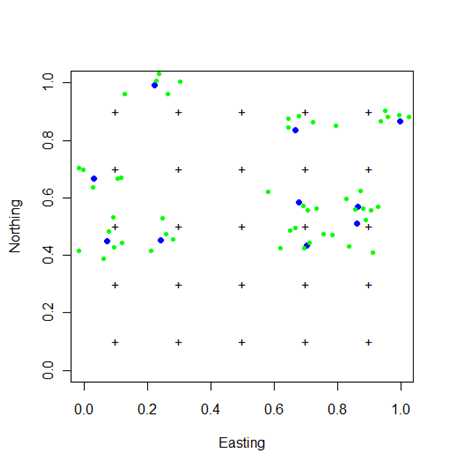
\includegraphics[height=3in]{Ch1/figs/northingeasting}
\end{center}
\caption{Population of $N$ individual home-range centers ($\bf s_i$,
  blue points) and locations during $K=5$ occasions ($\bf u_{ik}$,
  black points). Crosses represent trap locations.}
\label{intro.fig.fig1}
\end{figure}



Although the full model including $u$ and $s$ fully describes the
ecological process, in practice we usually work with reduced forms of
this model. Examples include:
of such models are:
\begin{enumerate}
\item[$\bullet$] Classical distance sampling
\item[$\bullet$] Spatial capture-recapture models with fixed arrays of traps
  \citep{efford:2004, borchers_efford:2008, royle_etal:2009ecol,
    royle_etal:2009jae, gardner_etal:2010ecol,royle_etal:2011jwm}
\item[$\bullet$] Search-encounter models \citep{royle_young:2008, royle_etal:2011mee}.
\item[$\bullet$] Capture-recapture distance-sampling \citep{borchers_etal:1998}.
\end{enumerate}
In some classes of models, components for ${\bf u}$ and ${\bf s}$ will be confounded.
e.g., if ${\bf s}$ are uniform in space and ${\bf u}$ is
a random draw from some distribution centered at ${\bf s}$, then we might as
well define ${\bf u}^{*}=\Pr({\bf u})=\int_{s} [{\bf u}|{\bf s}][{\bf
  s}]ds$ which will itself by uniform
for reasonable choices of $[{\bf u}|{\bf s}]$.  Some examples
of typical spatial capture-recapture models and how
these various model components are manifest in specific cases is
described as follows:
\begin{itemize}
\item[1.] {\bf Distance sampling -- } The last 2 stages of the hierarchy
  are confounded (implicitly) and so analysis is based on the model
  $[y|u*] [u*]$. The ``process model'' is that of ``uniformity'': ${\bf u}^{*}
  \sim Unif({\cal S})$. Sometimes it is argued that distance sampling
  estimators are ``pooling robust'' which is a way of saying they are
  (or may be)
  relatively insensitive to this assumption. That may be true, but the
  construction of distance sampling estimators makes explicit the
  uniformity assumption as a mathematical fact.

\item[2.] {\bf Spatial capture-recapture model with a fixed array of traps} --
SCR models appear to have little in common with distance sampling
because observations are made only at a pre-defined set of discrete
locations -- where traps are placed. However, the models are closely
related in terms of our hierarchical representation above\footnote{Really
they're kind of like point-count distance sampling where the identity
of individuals is preserved across point samples , and distance is a
latent variable. i.e., SCR-DS. I feel like this point should be
emphasized somehow. Here? Later?}
In SCR models based on fixed arrays,
we cannot estimate both
$\Pr(y=1|{\bf u})$ and $\Pr({\bf u}|{\bf s})$ -- the probability  that
an individual ``moves to ${\bf u}$'' cannot be seperated from the
probability that it is detected given that it moves to ${\bf u}$,
because of the fact that the observation locations are fixed by
design.
Formally, such SCR models confound $[y|{\bf u}]$  with $[{\bf
  u}|{\bf s}]$ so that the observation model arises as:
\[
 [y|{\bf s}] = \int_{u} [y|{\bf u}][{\bf u}|{\bf s}] du
\]
This confounding happens because SCR sampling is spatially biased -
restricted to a fixed pre-determined set of locations.

Conversely,
distance sampling confounds $[{\bf u}|{\bf s}][{\bf s}]$ because, essentially, there is
only a single realization of the encounter process.

It is probably
reasonable to assume that $\Pr(y=1|{\bf u})=1$ or at least it is locally
constant for most devices (e.g., cameras, etc..), and thus the
detection model will have the interpretation in terms of movement (see
chapter XXX.YY).

\item[3.] {\bf Search-encounter models -- } What we call
  ``search-encounter'' models \citep{royle_etal:2011mee}
  are kind of a hybrid model - combining features of SCR models and
  features of distance sampling. Like distance sampling they allow for
  encounters in continuous space which provide direct observations
  from $[{\bf u}|{\bf s}]$.
Thus, the
  hierarchical model is fully identified.

\item[4.] {\bf Capture-recapture/distance-sampling -- } See
  \citet{borchers_etal:1998}. As with the search-encounter models the
full hierarchical model is identified:
$[y|{\bf u}][{\bf u}|{\bf s}][{\bf s}]$ but the quantities don't
really mean the same thing as before.

To understand this, we expand the model to accommodate imperfect
measurements of ${\bf u}$. Let ${\bf u}_{obs}$ be an observation of
${\bf u}$ (i.e., made with error). A larger hiearchical model is this:
\[
[y|{\bf u}][{\bf u}_{obs}|{\bf u}][{\bf u}|{\bf s}][{\bf s}]
\]
If we make replicate ``instantaneous'' observations of location, then
information is provided about
 $[{\bf u}_{obs}|{\bf u}]$ (i.e., measurement error). However, in a normal
 distance sampling application, with instantaneous sampling, we don't
 learn anything about $[{\bf u}|{\bf s}]$,
in effect, we are again confounding $[{\bf u}|{\bf s}]$ and $[{\bf
  s}]$: ${\bf u}^{*} = \int_{s} [{\bf u}|{\bf s}][{\bf s}] ds$. So the CR-DS model focuses on:
\[
[y|{\bf u}^{*}][{\bf u}_{obs}|{\bf u}^{*}][{\bf u}^{*}].
\]
Structurally, this is the same basic model as the search-encounter
model notwithstanding (1) that it is usually talked about in terms of
repeated measures of distance instead of location and (2) the 2nd
component of the hierarchy is not movement (an ecological process) but
rather ``measurement error'' and (3) the third component is not a home
range center but rather a movement outcome (``instantaneous
location'').  Thus, while the models are structurally identically, the
meaning and interpretation of quantities are distinct.

%These are
%mostly all semantic and conceptual distinctions which are easy to
%define in a convenient table:
%\begin{table}[ht]
%\centering
%\title{What things mean in each model.}
%\begin{tabular}{c|cc}
%           &   Search encounter models     &  CR-DS  \\  \hline
%  $\sigma$    &  movement       &   measurement error  \\
% ${\bf s}$ & activity center & instaneous location \\
%\end{tabular}
%\end{table}
\end{itemize}

Efford's characterization:
proximity detectors, multi-catch, single-catch, etc....
acoustic detectors, ....

\section{Analysis of spatial capture-recapture models}



\begin{comment}
\subsection{Models don't have political views!}

Whereas hierarchical modeling is a conceptual and framework for
formulating models, the method of inference is independent of model
formulation. Hierarchical models can be analyzed by Bayesian and
non-Bayesian methods. A model is not Bayesian or frequentist -- what
you do to that model is Bayesian or frequentist!
\[
\bullet \mbox{"Hierarchical model"} \ne  \mbox{"Bayesian"}!!!
\]
Thus, analysis of hierarchical models is easily achieved using either
Bayesian or classical (likelihood, frequentist) methods. By
``analysis'' we mean any type of estimation, characterization of
uncertainty, prediction, model selection, or evaluation and we are not
dogmatic about our choice of inference methods. That said, we do
recognize a benefit of the Bayesian approach which is that it
emphasizes model construction and not the construction of
procedures. The Nobel prize\footnote{called something else besides
  Nobel, officially} winning econometrician Christopher Sims (Slides
from the Hotelling Lecture 6/29/2007 at Duke University - cite his
webpage) said it this way: ``Bayesian inference is a way of thinking,
not a basket of 'Methods''' Conversely, ecologistis that are subjected
to a classical statistical curriculum often have only a vague sense of
what the model is that any particular procedure is employing.  We
agree with Little \citet{little:2006}
that there should be more emphasis on understanding statistical
modeling, and less emphasis on statistical methods.  Toss the ``basket
of methods'' out the window and learn how to model!

\end{comment}

We rely strictly on principles and procedures of {\it parametric
  inference} in our analysis of hierarchical models in general and,
specifically, of spatial capture-recapture models. Parametric
inference is that in which we make explicit probability assumptions
about how the data were generated. Inference procedures are then
developed under the assumption that the model is truth, because formal
parametric inference procedures that we understand the joint
probability distribution of everything that is a realization of a
random variable. {\bf There is something missing in the previous sentence. require, maybe?}There are two popular flavors of parametric
inference: {\bf Classical inference}: The joint probability distribution
of observations is the {\bf likelihood}. We maximize it to obtain MLEs
and do other fun things to it. We evaluate procedures by thinking
about what would happen over replicate realizations of data to which
our procedures are applied.  {\bf Bayesian inference} is based on the
posterior distribution, which is the joint probability distribution of
the data and also parameters and possibly other quantities including
latent variables or random effects.

Because SCR models contain a collection of latent variables - random
effects -- a natural framework for classical analysis of the models is
based on integrated likelihood \citep{laird_ware:1982,berger_etal:1999}. That is, while
the observation model is conceptualized conditional on the random
effects (the locations of individuals), classical inference is
formally based on the likelihood constructed from the {\it marginal}
probability distribution of the observations (i.e., {\it
  unconditional} on the random effect). The random effects are removed
from the conditional likelihood by integration (which is accomplished
numerically in spatial capture-recapture models). This approach to
inference has been formalized in the context of SCR models by
\citet{borchers_efford:2008, efford:2011}, and implemented for some
classes of models in the software package {\bf DENSITY} \citep{efford:2004}
and the {\bf R} package \mbox{\tt secr} \citep{efford:2011}.

Bayesian analysis is another natural framework for the analysis of
models containing latent variables or random effects.  Under this
approach, analysis of the model is based on Monte Carlo simulation
from the posterior distribution, which is the product of the
conditional likelihood, the distribution of the random effects, and
perhaps other distributions.  This approach was developed by
\citet{royle_young:2008}, and was motivated by work focused on
modeling individual effects in capture-recapture models. In
particular, a convenient reparameterization of individual covariate
models can be obtained using a method known as data augmentation
\citep{royle_etal:2007}, see \citet{royle:2008} for an application to
classical individual covariate models in \citet{royle:2008}. The close
similarity between individual covariate models and spatial
capture-recapture models, with the individual's activity center ${\bf
  s}$ being the individual covariate, led to the application of the
data augmentation method described by \citet{royle_young:2008} and subsequent papers.

These two technical formulations (classical inference based on
integrated likelihood and Bayesian inference) both provide rigorous solutions to
the inference problems posed by spatial capture-recapture data.  There
are also minor distinctions to be aware of. For example,
as a technical matter, \citet{borchers_efford:2008} and related work, assume
a Poisson point process that is unconditional on $N$ whereas Royle and
Young (2008) and related work assume a binomial point process model
which is conditional on $N$.
%More importantly, Borchers and Efford
%develop the analysis in a way that is unconditional on the point
%process (which is removed from the conditional likelihood by
%integration).  Conversely, the analysis of \citet{royle_young:2008} is
%conditional on the underlying point process. As a technical matter,
%Bayesian analysis allows us to analyze the model that is conditional
%on the underlying point process and will otherwise have more
%flexibility - open populations, using telemetry data, etc.. as will be
%demonstrated in later chapters.

We tend to favor Bayesian inference for conceptual and philosphical
reasons but we also think that  integrated likelihood
for complex point process models may prove difficult. On the other
hand, we suspect that Bayesian
analysis by MCMC
of the model that is conditional on the underlying point process will
prove to be more versatile and generalizable for complex point process
models. We say this only
tentatively and throughout this book we are not exclusive in our views
of inference and use Bayesian and classical methods of inference
interchangeable and opportunistically in this book.
We don't want to get too much into the technical foundations of
Bayesian analysis because there are many good books now including
\citet{link_barker:2009}.  \citet{kery:2010, mccarthy:2007,
  king_etal:2009} and probably others by the time this book is
finished. That said,  Bayesian analysis is introduced at a
level required to get through this book in Chapter 2.


\subsection{Implementing hierarchical models}

In our experience, students in ecology and even many established
scientists simply cannot separate what they need to do from how to do
it.  They cannot distinguish clearly (either conceptually or actually)
the difference between the model for their data, and the actual
procedure of how to estimate parameters of that model, or make
predictions - ie., how to do the calculations. Sometimes this issue
raises itself in an email from some hapless grad student wondering
``what is the right statistical test for this type of data?''  In a
sense it is this view that drives our approach to developing elements
of this book.

In contemporary statistical ecology, models and methods are sometimes
obscured by named procedures often that are completely uninformative,
the technical details of which hide in obscurity in some black boxes
such as MARK, PRESENCE, DISTANCE, etc., known only by the few
specialist experts in the field. While it is sometimes convenient to
refer to a type or class of models by a name (logistic regression or
even ``model Mh'') in order to emphasize a broad concept or
methodological area, this is only useful if the fundamental
statistical and mathematical structure underlying that name is
clear. As such, we try to focus on model development and keep the
model development distinct from how to combine our data with the model
to produce estimates and so forth. We talk a lot about hypothetical
data we wish we could observe - complete data sets - data sets as if
$N$ were known, etc.. We talk about the model in precise terms and
then break down various ways for analyzing the model either using
likelihood methods or Bayesian methods or some black-box that does one
or the other.

To fit models, we rely heavily on the various implementations of the
{\bf BUGS} language including {\bf WinBUGS} \citep{lunn_etal:2000},
{\bf JAGS} \citep{plummer:2003}
 and {\bf OpenBUGS} \citep{thomas_etal:2006}. We really like
the {\bf BUGS} language, not merely  as a computational device for
fitting models but because it emphasizes
understanding of what the model is and fosters understanding how to
build models - as Kery XYZ XYZ says ``it frees the modeler in you.''  (direct
citation for this would be nice).  However, in addition to using the
{\bf BUGS} language and its various implementations, we also develop our own
{\bf R} code both for doing MCMC
and maximum likelihood, for which we also use the R
package \mbox{\tt secr} \citep{efford:2011}. In addition, we have
created an {\bf R} package to go with this book, \mbox{\tt scrbook},
which contains the data sets, {\bf R} and {\bf BUGS} scripts, and {\bf
  R} code for doing summary analyses, and some likelihood and MCMC
functions written solely in {\bf R}.


\subsection{SCR models as GLMMs}

Most SCR models covered in this book
have a formulation that closely resembles generalized linear
models (GLMs) in which the individual activity centers appear as a
random effect \citep{royle_etal:2009ecol, royle_gardner:2011}. That is,
they appear conceptually and structurally similar to so-called
generalized linear {\it mixed} models (GLMMs) which are pervasive in
the literature of many disciplines including ecology.  This actually
has, we think, some profound consequences both conceptually and
practically (in terms of implementation). For example, as a result,
SCR models should by conceptually accessible to practitioners with
some basic statistical understanding and experience.  And, we believe
that practitioners will have some flexibility in developing models
that fit their specific situation. Quite simply - given existing
software, it is easy for practitioners to specify models, even if they
lack the technical know-how to devise their own fitting routines.







\section{Criticisms of Spatial Capture-Recapture Models}

By this point we hope you are convinced that spatial capture-recapture models
offer numerous advantages over their non-spatial
counterparts. However, we have frequently used the terms
``assumptions'' and ``priors'', which make some people feel
uneasy. Our view is that expressed eloquently by Link (ADD
QUOTE). Furthermore, we note that hierarchical models allow us to
modify any assumption deemed too
restrictive. That is, we can always generalize our models given enough
data. Chapter is a classic example because it addresses
perhaps the most common criticism of SCR, that ``real animals'' don't
have symmetic home ranges. In fact people have written entire papers
beating up on SCR because they \emph{assume} that this the bivariate
normal model for the encounter processes is a rigid requirement of SCR
methods. Although we believe this assumption is quite reasonable in
many contexts, Chapter \ref{chapt.ecoldist} clearly illustrates that
alternatives exist, and that SCR provides a rigours framework for
testing for departures from this assumption, and even evaluating
hypotheses that may explain why animals move the way they do.



\message{ !name(Ch1b.tex) !offset(-788) }
